\chapter{結果と考察}
本章では，symmergent重力の整合性を一般相対論とEHTの観測データとの比較を通して検証する．

\section{symmergent重力と一般相対論の比較}
\cite{Gkigkitzis:2014cla,Calmet:2024pve,Kuntz:2017pjd,Dragasevic:2025mtf,}
symmergent重力および一般相対論のブラックホールの有効ポテンシャルを解析した結果を示す．\zcref{fig:potential}は有効ポテンシャルと距離の関係を表したグラフである．
\begin{figure}
    \centering
    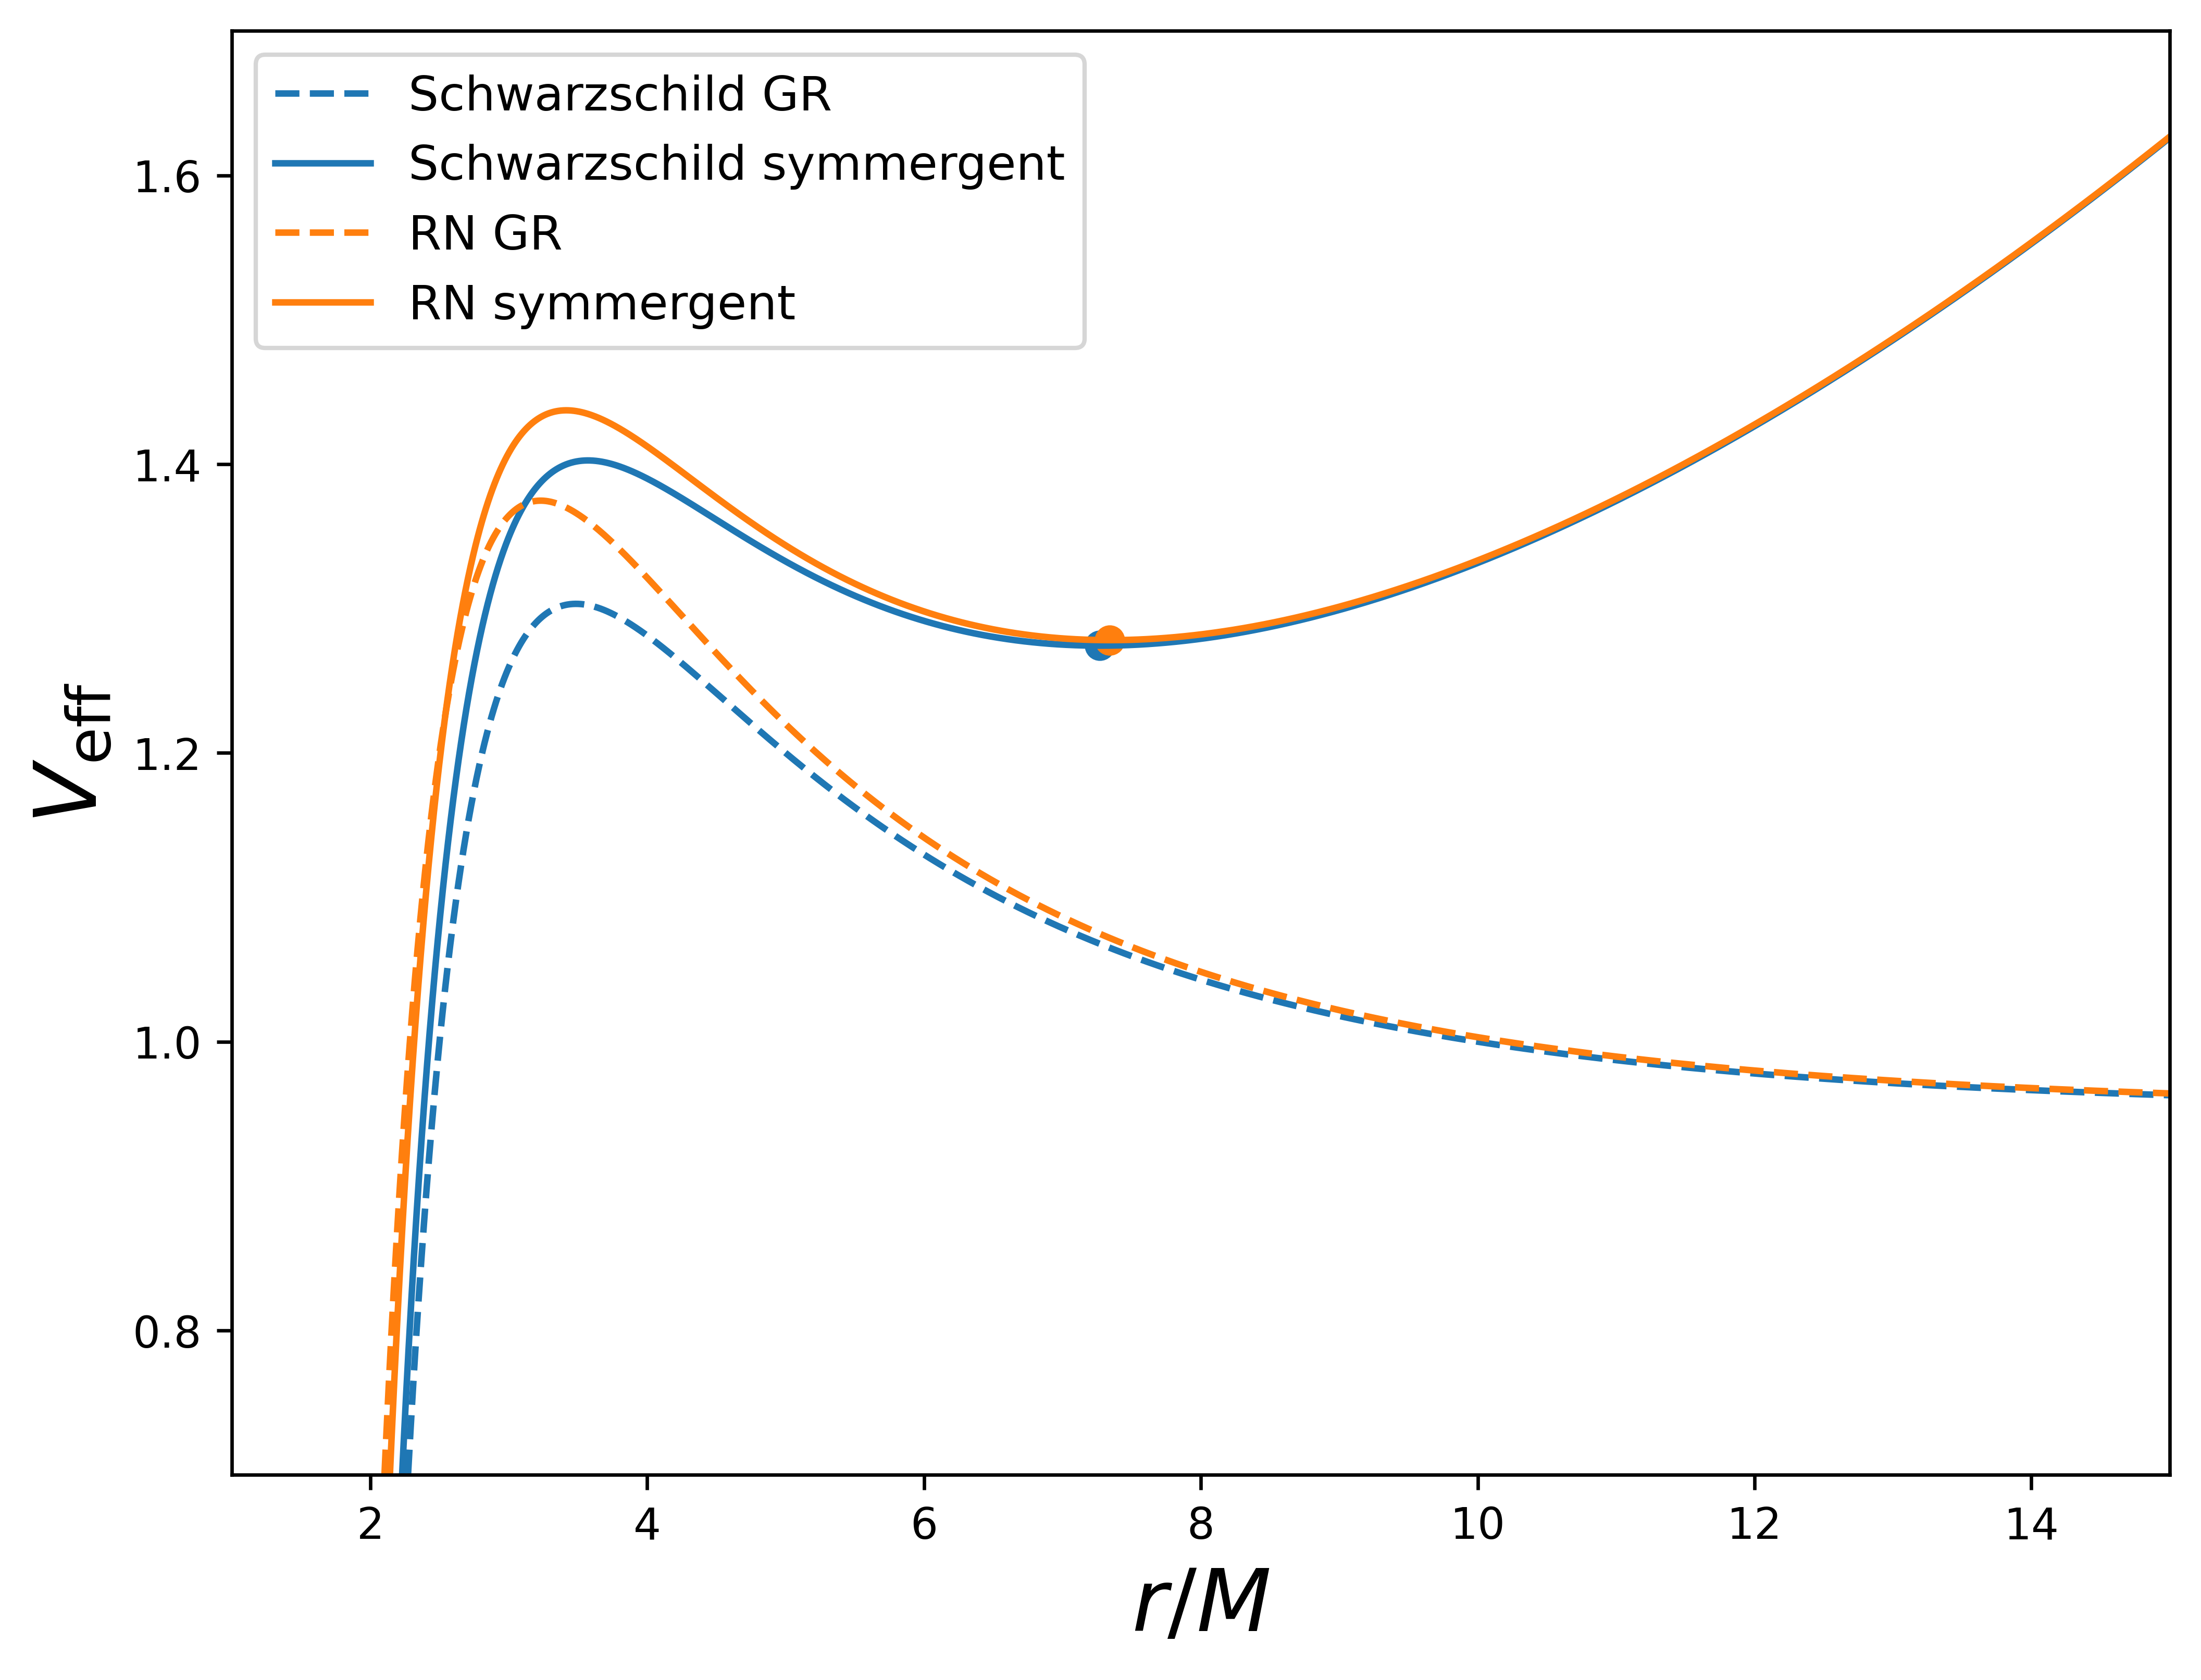
\includegraphics[width=1\textwidth]{potential.png}
    \caption{ブラックホールの有効ポテンシャルとブラックホールまでの距離の関係．ブルー色はSchwarzschild，オレンジ色はRN．実線はsymmergent重力，破線は一般相対論を表す．($M=1.0, G=1.0, \mathcal{L}=5.0, \theta=\pi/2, \alpha=0.9, c_O=-0.5, q=0.5$)}
    \zlabel{fig:potential}
\end{figure}
\zcref{fig:shadow}はシャドウ半径と距離の関係を表したグラフである．
\begin{figure}[h]
    \centering
    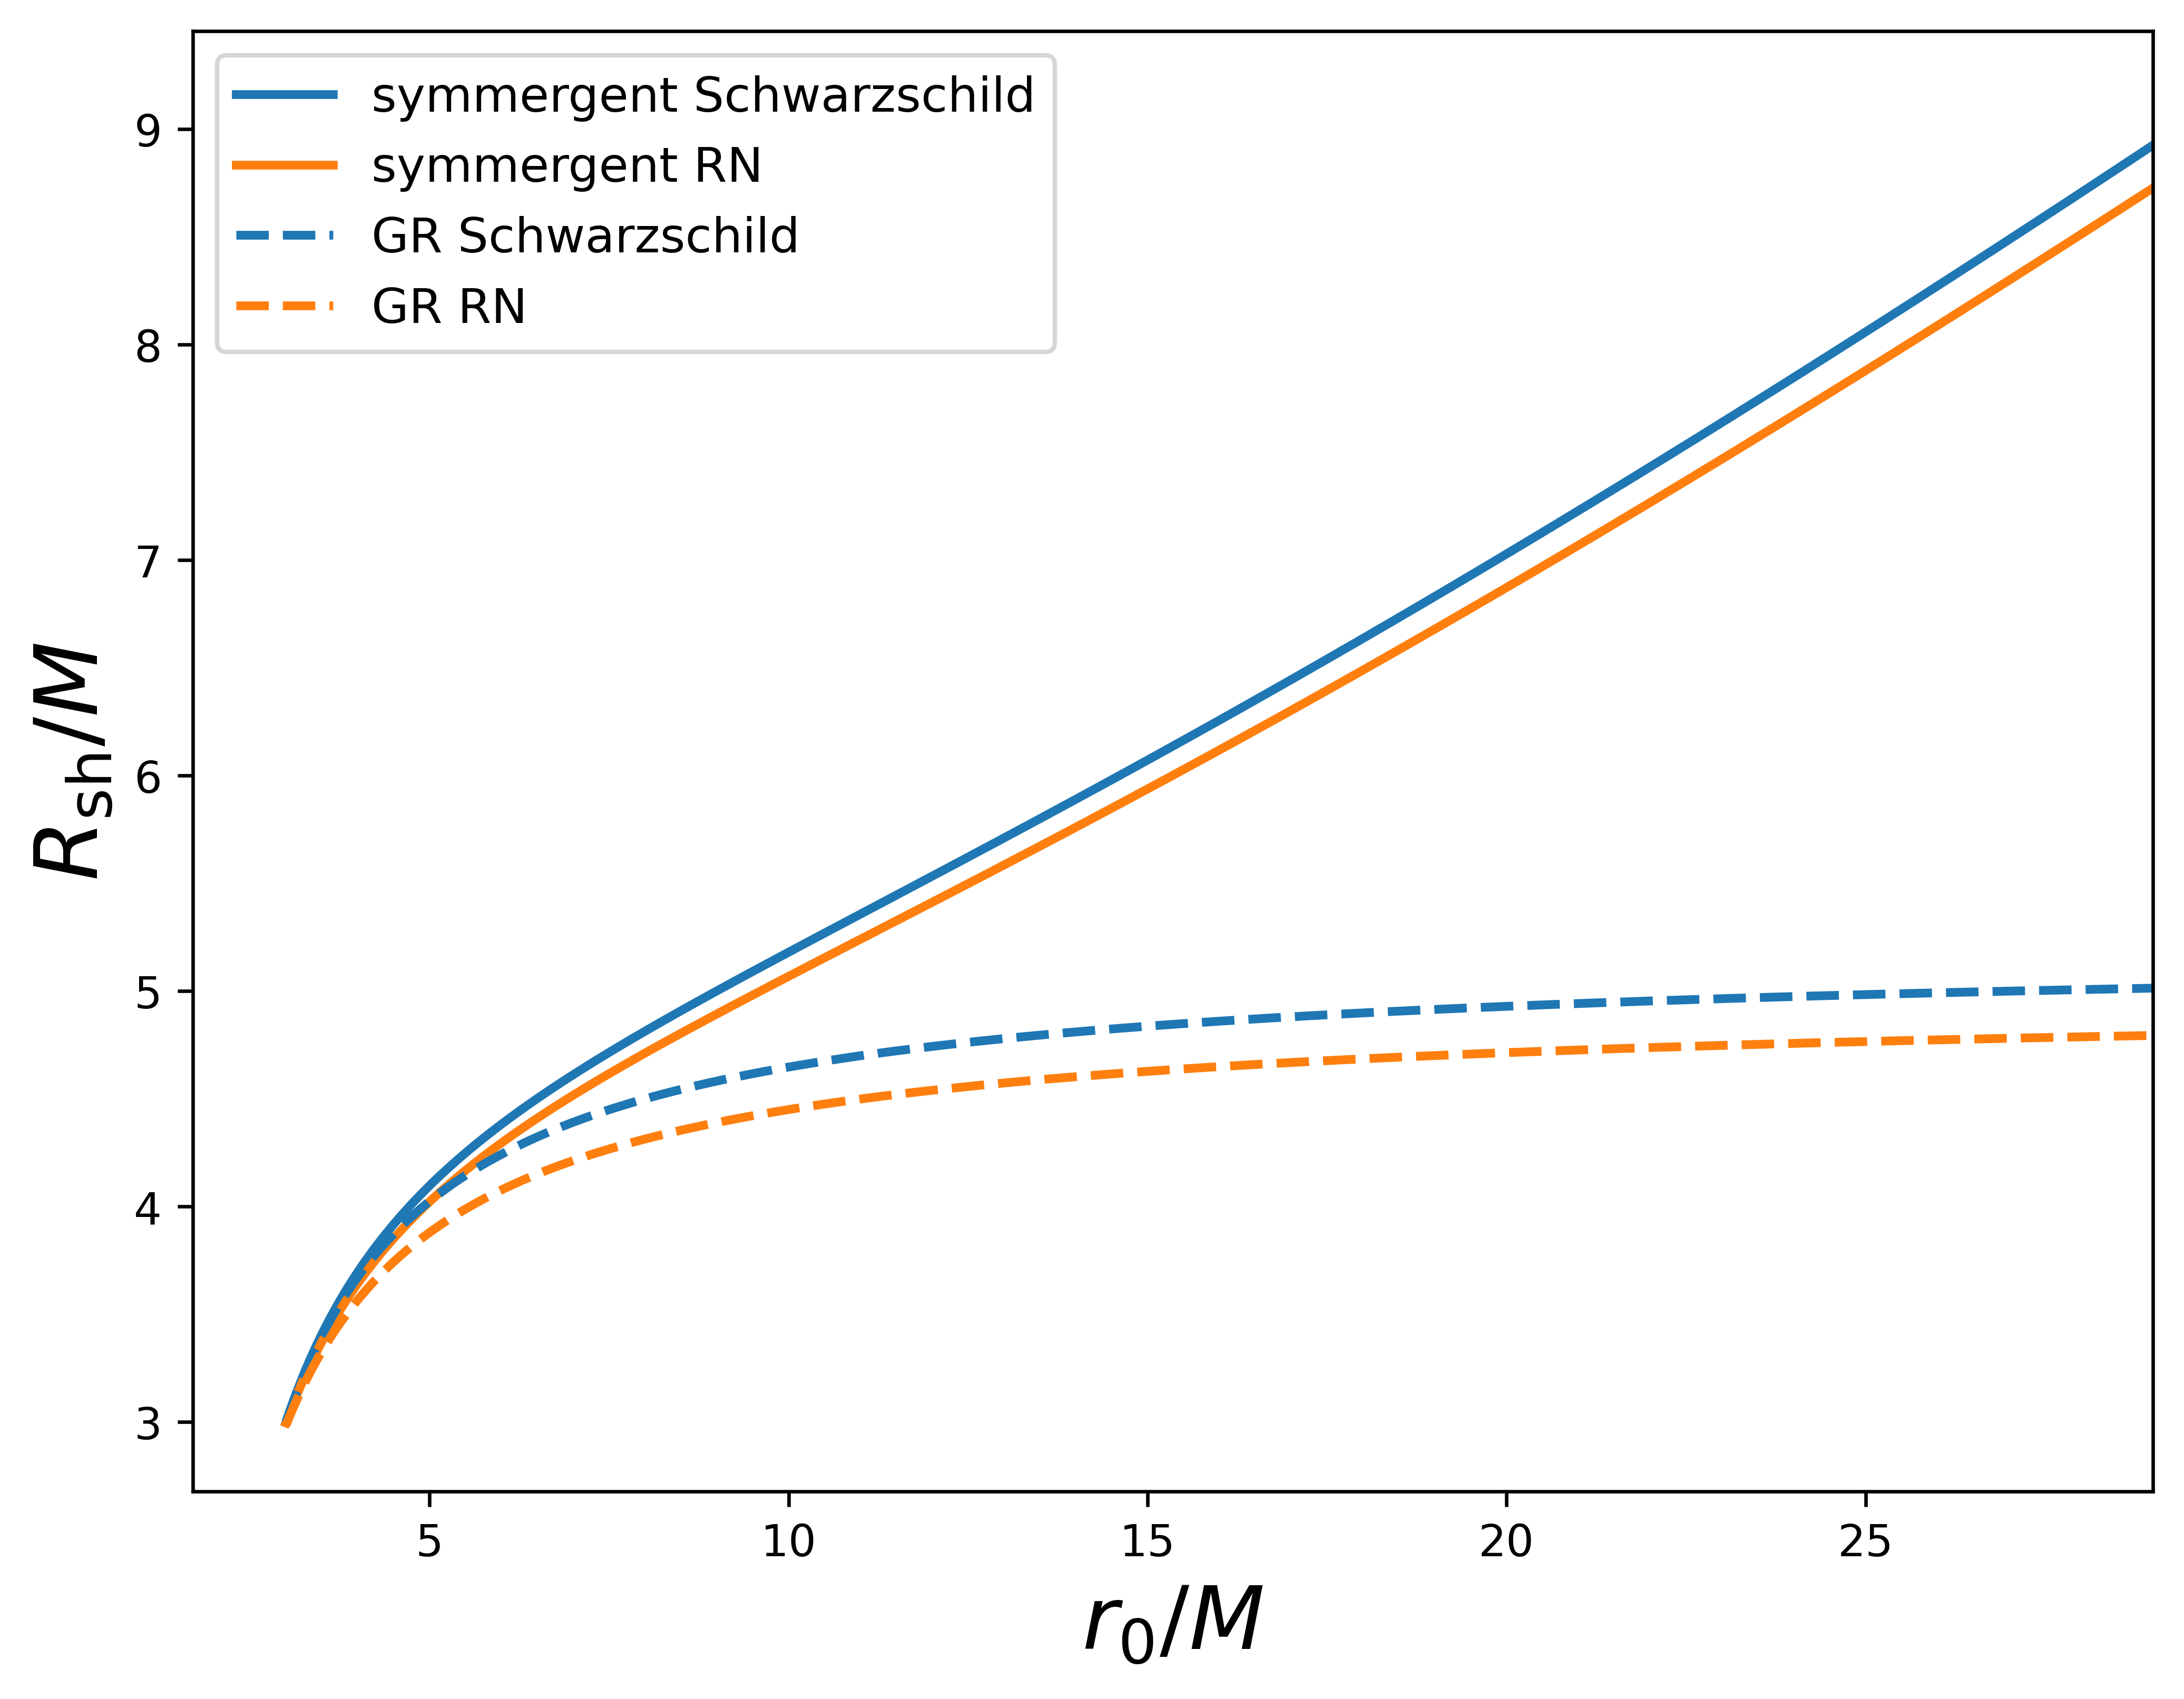
\includegraphics[width=1\textwidth]{shadow.png}
    \caption{ブラックホールシャドウ半径とブラックホールからの距離の関係．ブルー色はSchwarzschild，オレンジ色はRN．実線はsymmergent重力，破線は一般相対論を表す．($M=1.0, G=1.0, \theta=\pi/2, \alpha=0.9, c_O=-0.5, q=0.5$)}
    \zlabel{fig:shadow}
\end{figure}

\section{EHTとの比較}
\begin{table}[tb]
    \caption{EHTの観測データ}
  \zlabel{tab:EHT}
  \centering
  \begin{tabular}{cccc}
    \toprule
    Black hole & Mass ($M_\odot$) & Angular diameter ($2\theta$) & Distance ($\mathrm{kpc}$) \\
    \midrule
    Sgr.A* & $4.3\pm 0.013\times 10^6$ & $48.7\pm 7$ & $8.277\pm 0.033$ \\
    M87* & $6.5\pm 0.90\times 10^9$ & $42\pm 3$ & 16800\\
    \bottomrule
  \end{tabular}
\end{table}
EHTによってSgr.A*とM87*にあるブラックホールが撮影された．\zcref{tab:EHT}はEHTから得られたデータの一部である．ブラックホールの質量$M$，視直径$2\theta$，ブラックホールまでの距離$D$が得られ，それらを用いてシャドウ直径$d_{\mathrm{sh}}$は以下のように与えられる．
\begin{dmath}
    d_{\mathrm{sh}}=D \theta/M
\end{dmath}
この式から観測範囲を設けることができる．
\begin{figure}[h]
    \centering
    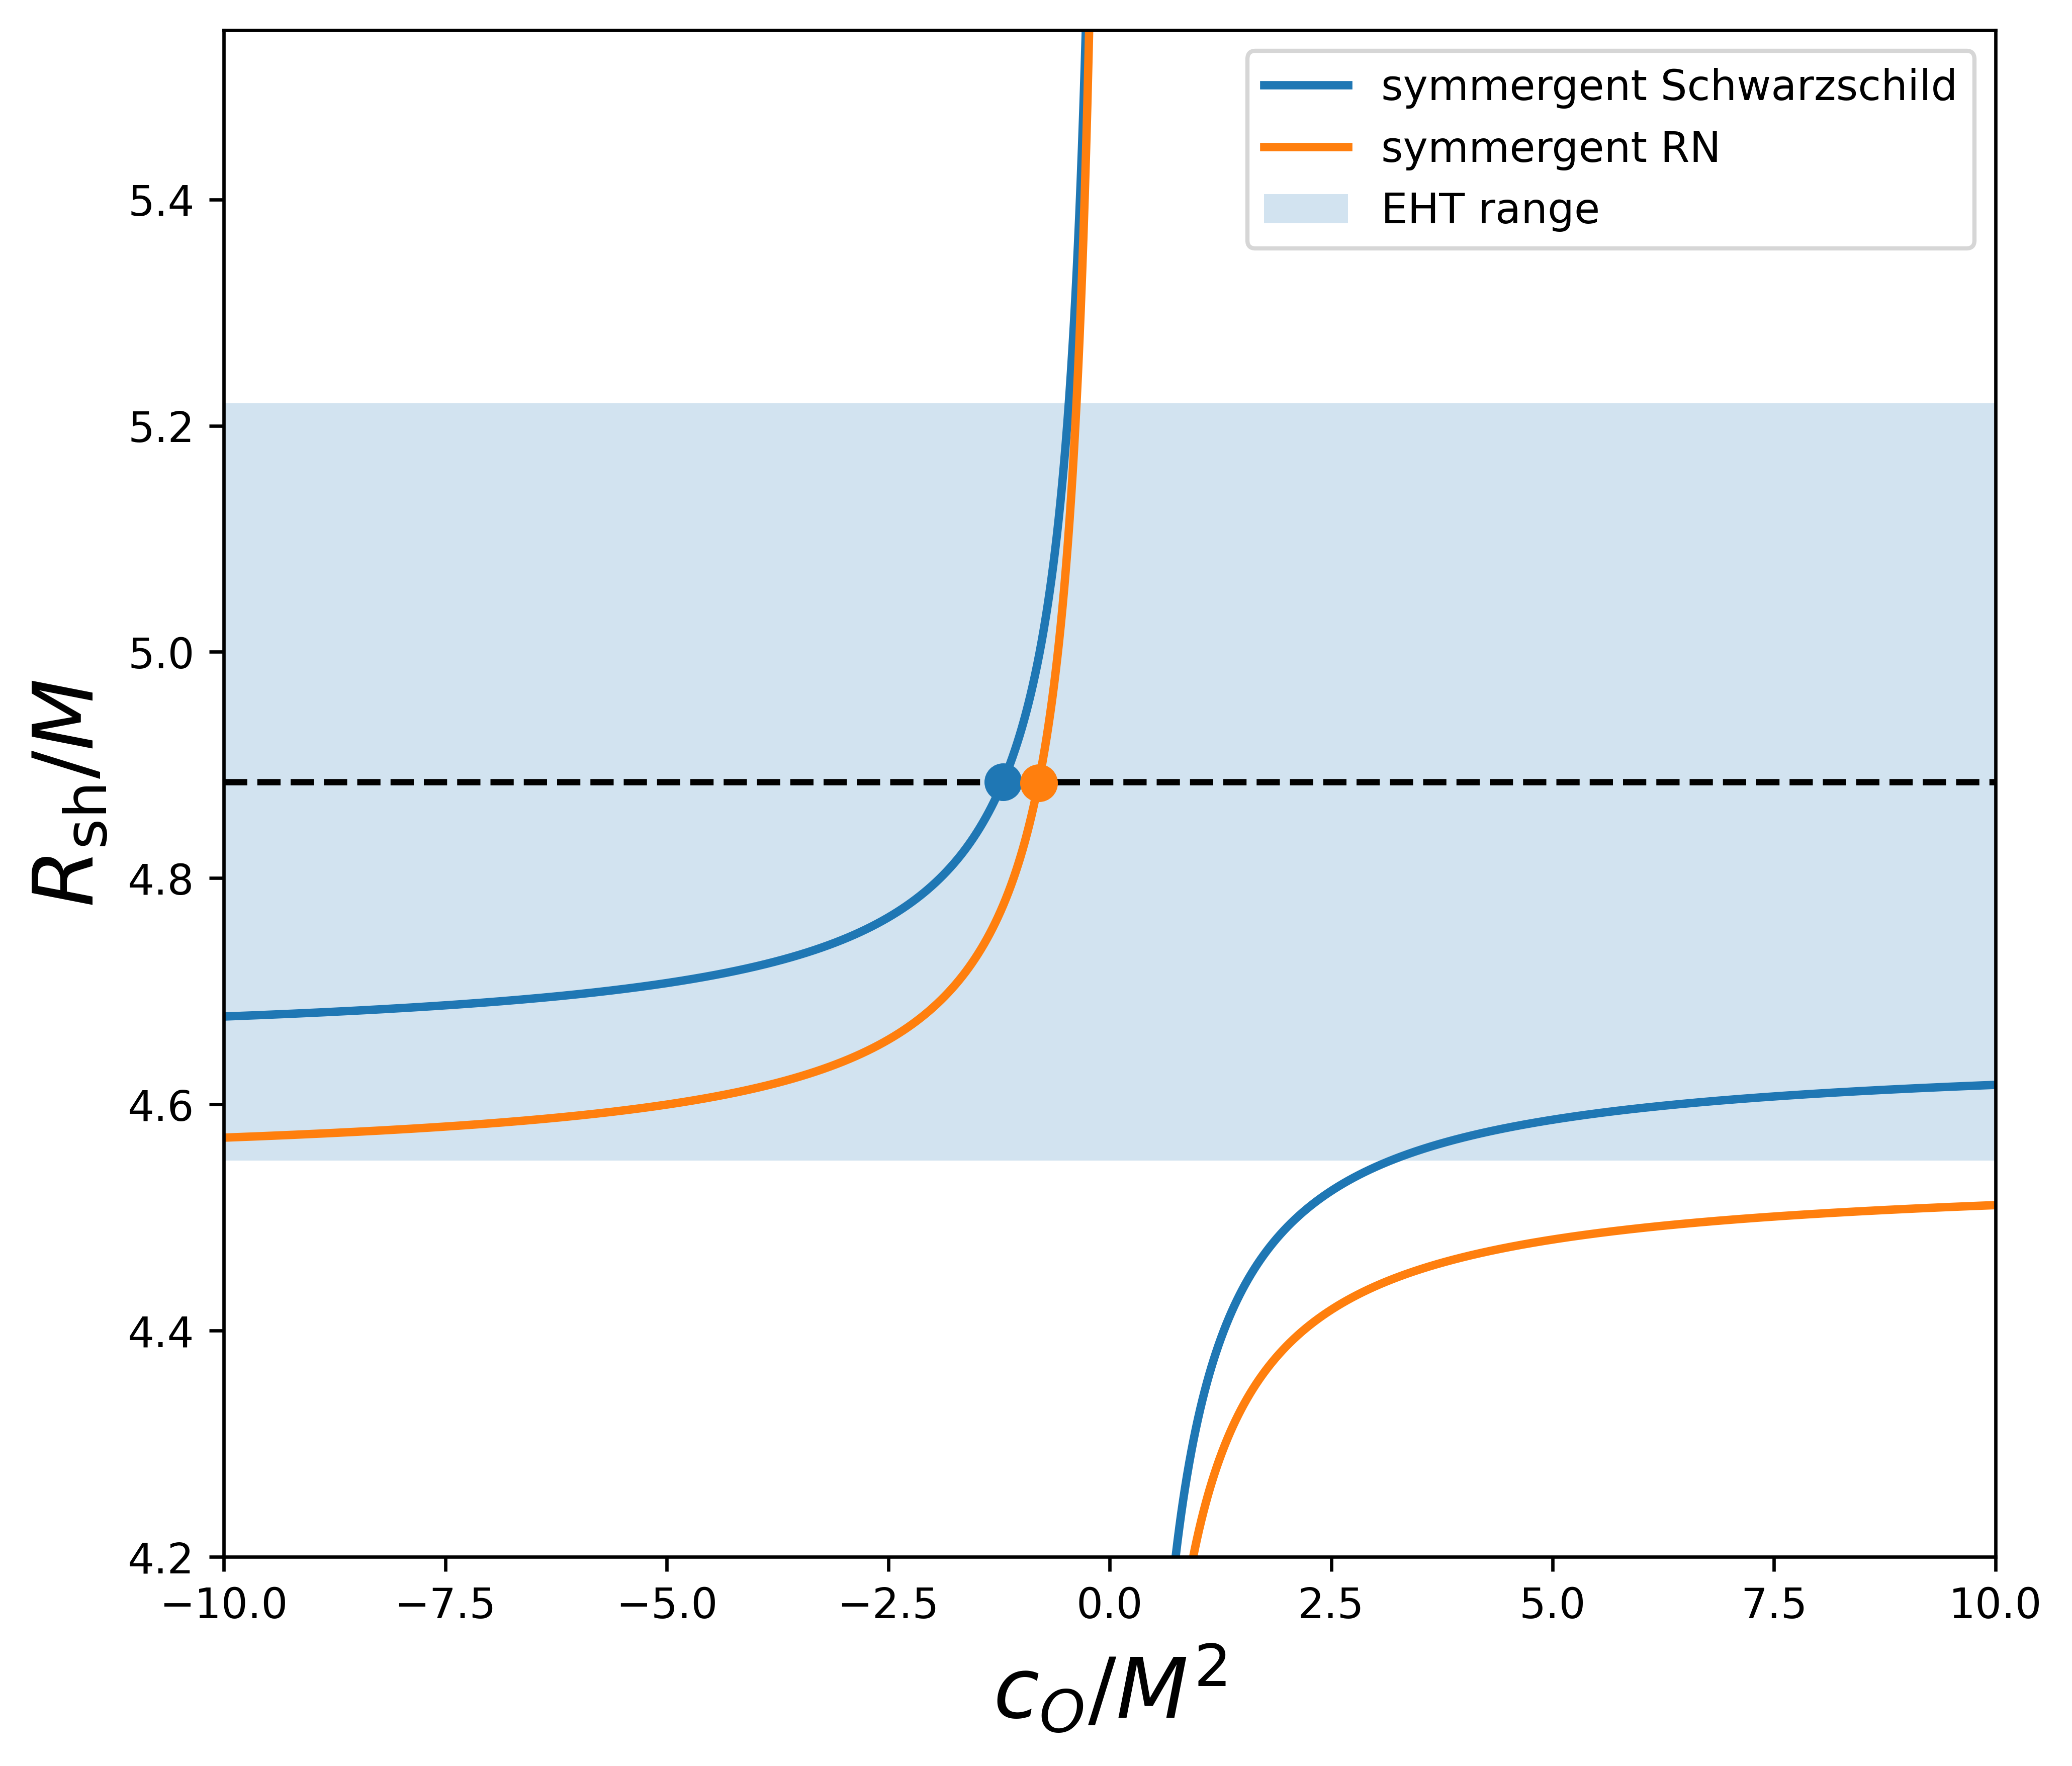
\includegraphics[width=1\textwidth]{sgrA.png}
    \caption{シャドウ半径とsymmergentパラメータ$c_O$の関係．帯状の範囲がSgr.A*の観測データから推定されるシャドウ半径である．ブルー色はSchwarzschild，オレンジ色はRNを表す．($M=1.0, G=1.0, \theta=\pi/2, \alpha=0.9, r_0=10.0, q=0.5$)}
    \zlabel{fig:sgrA}
\end{figure}
\begin{figure}[h]
    \centering
    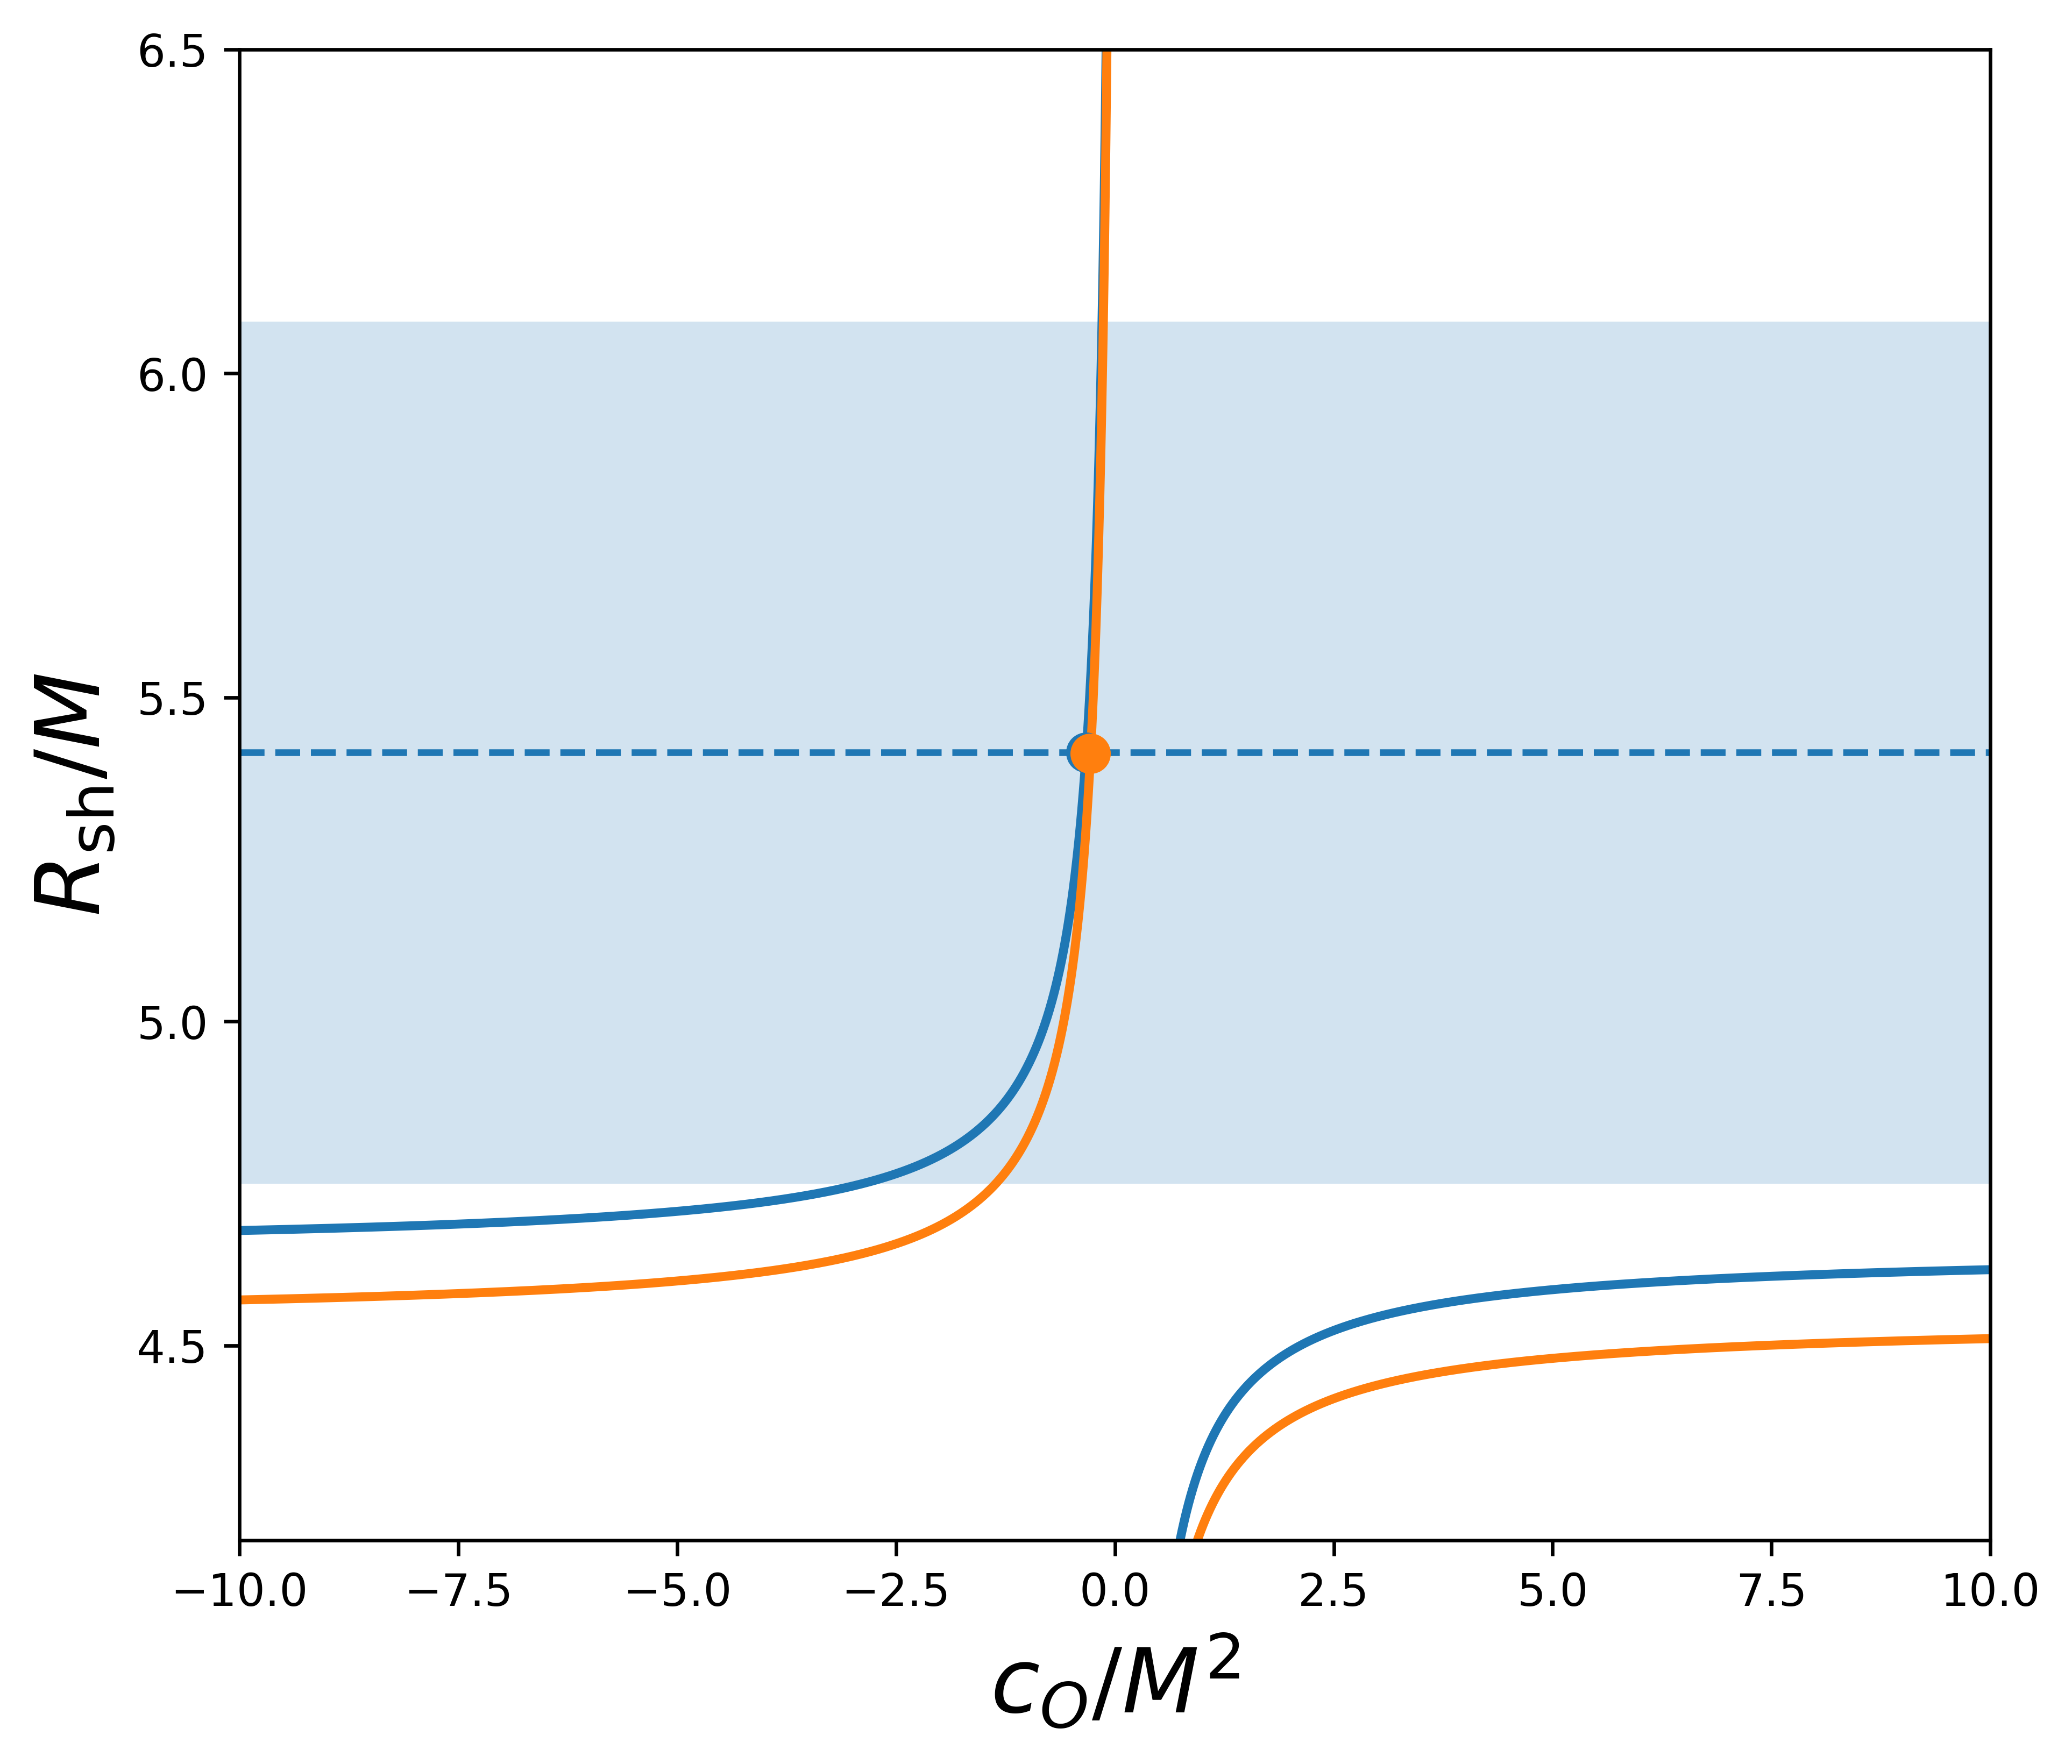
\includegraphics[width=1\textwidth]{M87.png}
    \caption{シャドウ半径とsymmergentパラメータ$c_O$の関係．帯状の範囲がM87*の観測データから推定されるシャドウ半径である．ブルー色はSchwarzschild，オレンジ色はRNを表す．($M=1.0, G=1.0, \theta=\pi/2, \alpha=0.9, r_0=10.0, q=0.5$)}
    \zlabel{fig:M87}
\end{figure}

\begin{table}[tb]
  \caption{例：主要パラメータ（単位は見出しに含める）．}
  \label{tab:params}
  \centering
  \begin{tabular}{lcc}
    \toprule
    Black hole & Schwarzschild & RN \\
    \midrule
    Sgr.A* & \num{70} & \unit{\kilogram\meter\per\second} \\
    M87* & 0.3 & --- \\
    \bottomrule
  \end{tabular}
\end{table}